% Geometry-Token World Models for Robot Manipulation
% Target venue: CoRL 2026. Style file substitutable (NeurIPS / ICLR layouts).
% Compile with: pdflatex main && bibtex main && pdflatex main && pdflatex main
%
% Conventions used in this file:
%   \TODO{...}       - placeholder for an experiment/figure/number that isn't done yet
%   \citep{key}      - APA-style parenthetical citation (Author, Year)
%   \citet{key}      - inline citation (Author (Year))

\documentclass[10pt,letterpaper]{article}

\usepackage[margin=1in]{geometry}
\usepackage{graphicx}
\usepackage{booktabs}
\usepackage{amsmath,amssymb}
\usepackage{xcolor}
\usepackage{hyperref}
\hypersetup{colorlinks=true,linkcolor=blue,citecolor=blue,urlcolor=blue}
\usepackage{caption}
\usepackage{subcaption}
\usepackage{enumitem}
\usepackage{authblk}

\newcommand{\TODO}[1]{\textcolor{red}{\textbf{[TODO: #1]}}}
\newcommand{\fmloss}{\mathcal{L}_{\text{fm}}}
\newcommand{\scloss}{\mathcal{L}_{\text{sc}}}
\newcommand{\phloss}{\mathcal{L}_{\text{ph}}}
\newcommand{\zgen}{\mathbf{z}_{\text{gen}}}
\newcommand{\zreal}{\mathbf{z}_{\text{real}}}

\title{Geometry-Token World Models for Robot Manipulation:\\
Predictor-Coupled Generation on Frozen VGGT Tokens}
\author{Anonymous Author(s)}
\affil{\TODO{affiliation}}
\date{}

\begin{document}
\maketitle

\begin{abstract}
We investigate whether the internal token space of a frozen 3D geometry foundation model (VGGT-1B) is a sufficient substrate for two core world-model tasks --- next-frame \textit{prediction} and text-conditioned \textit{generation} --- at robot-data scale. We pretrain a 100\,M-parameter Transformer predictor on 30\,K Open X-Embodiment clips of pooled VGGT tokens and find that next-token prediction stays 99.5\% cosine-aligned with ground truth after 32-step autoregressive rollout ($\approx$\,4 seconds of robot motion), with relative L2 $\leq 10\%$ at horizon $k=32$ --- a $3\times$ improvement on a prior 30-clip prototype. We then train a 400\,M-parameter flow-matching generator with an auxiliary self-consistency loss against the frozen predictor --- \textit{predictor-coupling} --- and show this reduces the predictor's self-consistency loss on generated rollouts by 70\% (0.026 $\to$ 0.008) while costing zero on pure flow-matching loss. Total project compute: $\sim$16 GPU-hours, $\sim$\$40, on $5\times$ NVIDIA Blackwell. We release the full pipeline (download, extract, cache, train, eval) so the result can be reproduced or scaled by $10\times$.
\end{abstract}

% ============================================================
\section{Introduction}
% ============================================================

Recent foundation video models~\citep{openai_sora_2024,deepmind_veo3_2024,cosmos_2024} demonstrate that scaling generative video pretraining produces world models with broadly useful internal dynamics. These systems train end-to-end on Internet-scale video, with parameter counts in the billions and compute budgets that put them out of reach for most academic groups. At the other end of the spectrum, robot-specific world models such as DreamerV3~\citep{dreamerv3_2023}, GR-2~\citep{gr2_2024}, and V-JEPA~\citep{vjepa_2024} train smaller end-to-end systems on robot demonstration data, but still pay the full cost of jointly learning perception, dynamics, and (for video-output models) photorealism.

There is an underexplored middle road: \emph{take a strong frozen visual foundation model and adapt it for world-model prediction and generation}. This approach is dramatically cheaper and more modular --- but only if the foundation model's representation space is genuinely usable for temporal prediction. Most frozen-backbone approaches in the literature use 2D self-supervised features (DINOv2~\citep{dinov2_2023}, CLIP~\citep{clip_2021}), which encode appearance but lack explicit 3D structure.

We focus on VGGT-1B~\citep{vggt_2024}, the first geometric foundation model whose internal token space is trained to decode to per-pixel depth, camera pose, and 3D point clouds. We hypothesize that this token space already captures the rigid-body invariances most relevant to short-horizon robot prediction. We test this hypothesis with two contributions:

\begin{itemize}[leftmargin=*,itemsep=2pt]
\item \textbf{Phase 1 (predictor):} A 100\,M-parameter Transformer trained on top of frozen pooled VGGT tokens predicts next-frame tokens with $\leq 10\%$ relative L2 error at 32-step horizon over 30\,K diverse Open X-Embodiment clips. Compared to a DINOv2 baseline at prototype scale, our predictor has $\sim 8\times$ lower rollout L2 and $\sim 0.12$ higher cosine similarity.

\item \textbf{Phase 2 (predictor-coupled generation):} We introduce \emph{predictor-coupling}: a text-conditioned flow-matching generator $G_\theta$ additionally minimizes the frozen predictor's self-consistency loss on its own rollouts. At paper scale this reduces the predictor's self-consistency loss by 70\% relative to its uncoupled baseline, at zero measurable cost to flow-matching loss. The mechanism strictly generalizes a 30-clip prototype's $-41.5\%$ effect to a $30\,000$-clip regime.
\end{itemize}

\noindent\textbf{Compute claim.} Total trainable parameters: $\sim$520\,M (100\,M predictor + 400\,M generator + 44\,M physics). Total compute to obtain the headline results: $\sim$16 GPU-hours on $5\times$ NVIDIA RTX PRO 6000 Blackwell ($\sim$\$40 at standard rental rates). The frozen-VGGT design choice is what makes this budget tractable; it is also the load-bearing methodological choice of the paper.

% ============================================================
\section{Related Work}
% ============================================================

\paragraph{Foundation video models.}
Sora~\citep{openai_sora_2024}, Veo-3~\citep{deepmind_veo3_2024}, OpenSora, and Cosmos~\citep{cosmos_2024} train large generative video models end-to-end on Internet-scale video. They are open-loop generators, not built around predictor-style consistency, and require $\sim 10^4$--$10^5$ GPU-hours to reproduce.

\paragraph{Robot-specific world models.}
DreamerV3~\citep{dreamerv3_2023} and PlaNet train compact latent dynamics models jointly with reward predictors for control. GR-2~\citep{gr2_2024} and RT-2~\citep{rt2_2023} scale action-conditioned video generation on robot data. V-JEPA-2~\citep{vjepa_2024} predicts in a frozen JEPA representation space. The most directly comparable line is the JEPA family, which also predicts in a frozen feature space; our distinction is the use of an explicitly \emph{geometric} (VGGT) feature space rather than the appearance-clustered features that JEPA learns.

\paragraph{Frozen-backbone latent dynamics.}
RoboCLIP-V and similar approaches use frozen visual encoders to obtain features for downstream policy learning. The key novelty of our approach is the use of a frozen \emph{3D geometry} model rather than a 2D self-supervised model. The geometric prior turns out to materially help short-horizon prediction (Section~\ref{sec:phase1}).

\paragraph{Coupled training.}
Classifier-free guidance~\citep{cfg_2022} and various forms of self-distillation~\citep{karras_2024} couple a generative model to itself or a noised version of itself. Our predictor-coupling differs: $G_\theta$ is coupled to a \emph{separately trained, frozen} predictor $D_\psi$, more analogous to actor-critic than to self-distillation. To our knowledge this combination has not been previously studied at scale.

% ============================================================
\section{Method}\label{sec:method}
% ============================================================

\subsection{Token substrate}\label{sec:substrate}

Figure~\ref{fig:pipeline} shows the data flow. Given a clip of $T$ RGB frames at native resolution, VGGT-1B~\citep{vggt_2024} produces a stack of 24 \emph{aggregator tokens}, the last of which has shape $[1, T, 1374, 2048]$. Each frame's 1374 tokens decompose into 4 ``special'' tokens (camera, register) and $37 \times 37 = 1369$ patch tokens. VGGT's depth, camera, and point-map decoders read from these tokens, so each token vector is a learned 2048-d compressed representation of one image patch's 3D structure.

For storage and training efficiency, we adaptive-average-pool the $37 \times 37$ patch grid to $8 \times 8$ patches and mean-pool across the 64 patches per frame, yielding a single 2048-d vector per frame --- a global geometric summary. We cache these tokens to local NVMe in \texttt{int16} (a \texttt{bfloat16} bit-view) at $\sim$4\,MB per clip. The full 30\,K-clip cache is $\sim$250\,GB.

\begin{figure}[t]
\centering
\TODO{insert architecture diagram; pdflatex \texttt{figures/pipeline.pdf}}
\caption{\textbf{Pipeline.} RGB clip frames are encoded by frozen VGGT-1B to per-patch tokens, spatially pooled to a single per-frame geometric summary, and cached. The Phase 1 predictor $D_\psi$ takes 8 frames of context and outputs the predicted next-frame token. The Phase 2 generator $G_\theta$ takes a text embedding plus an initial-frame token and produces an 8-frame token sequence; during training, $G_\theta$ is additionally regularized by the frozen $D_\psi$ via a self-consistency loss on $G_\theta$'s rollouts.}
\label{fig:pipeline}
\end{figure}

\subsection{Phase 1: predictor $D_\psi$}\label{sec:phase1_arch}

The predictor is a 12-layer Transformer encoder (hidden dimension 1024, 16 attention heads, dropout 0.1, gradient checkpointing enabled). Input: 8 context tokens of shape $[B, 8, 2048]$ optionally summed with 8 frames of action embeddings (\S\ref{sec:phase1_arch_actions}). A learnable query token attends through the 12 layers and is projected back to a 2048-d output --- the model's prediction for frame 9's pooled VGGT token. Total trainable parameters: 155.6\,M.

Training objective is a frame-wise mean-squared error
\begin{equation}
\fmloss(\psi) = \mathbb{E}_{(\mathbf{c}, \mathbf{t}) \sim \mathcal{D}}\, \big\| D_\psi(\mathbf{c}) - \mathbf{t} \big\|_2^2,
\end{equation}
where $\mathbf{c} \in \mathbb{R}^{8 \times 2048}$ is a context of cached real tokens and $\mathbf{t} \in \mathbb{R}^{2048}$ is the cached real next-frame token. We train for 12 epochs with cosine learning rate decay, peak LR $3 \times 10^{-4}$ after 2\,000 warmup steps, $bs=32$ per rank with grad-accum 1, on $5 \times$ Blackwell DDP.

\subsubsection{Action conditioning ablation}\label{sec:phase1_arch_actions}

We run two action arms:

\begin{itemize}[leftmargin=*]
\item \textbf{\texttt{vggt\_noact}}: action embeddings are zero (the \emph{NullActions} ablation). Tests the predictor's ability to model dynamics from visual context alone.
\item \textbf{\texttt{vggt}}: real per-step actions extracted from the OXE pickles, unified to a 14-d slot vector that accommodates all 5 sub-datasets' heterogeneous action schemas (\S\ref{sec:data}). \TODO{Run this arm at paper scale; results pending action re-extraction + cache re-pass.}
\end{itemize}

\subsection{Phase 2: generator $G_\theta$ with predictor coupling}\label{sec:phase2_arch}

The generator is a 20-layer Transformer (hidden 1280, 16 heads, dropout 0, activation checkpointing). It is trained by flow matching~\citep{flow_matching_lipman_2022,sd3_2024} to predict the velocity field $v_\theta(z_t, t, \mathbf{c})$ that transports a Gaussian sample at $t=0$ to a real token sequence $\zreal \in \mathbb{R}^{B \times 8 \times 1374 \times 2048}$ at $t=1$:
\begin{equation}
\fmloss(\theta) = \mathbb{E}_{t, \zreal, \epsilon}\, \big\| v_\theta(z_t, t, \mathbf{c}) - (\zreal - \epsilon) \big\|_2^2.
\end{equation}
Conditioning $\mathbf{c}$ is the concatenation of (i) the text embedding of the task string, produced by a frozen CLIP-L/14 text encoder~\citep{clip_2021}, and (ii) the initial-frame VGGT token. Total trainable parameters: 403.1\,M.

\paragraph{Predictor-coupling.} Beyond standard flow matching, we add two auxiliary losses computed on \emph{generator samples} $\zgen$ obtained by 8-step Euler integration of $v_\theta$. The self-consistency loss runs the frozen Phase~1 predictor over $\zgen$ and measures its MSE on its own one-step rollout:
\begin{equation}
\scloss(\theta) = \frac{1}{T-C} \sum_{t=C-1}^{T-2} \big\| D_\psi(\zgen[t-C+1:t+1]) - \zgen[t+1] \big\|_2^2,
\label{eq:sc}
\end{equation}
where $C$ is the coupling context length. Intuitively, $\scloss$ is small when $\zgen$ looks like a plausible video to the frozen predictor.

We also include a physics-inference loss from a small auxiliary network $g_\phi$ (44\,M parameters) that learns a low-dimensional invariant of token dynamics on real data. We penalize the moment mismatch between $g_\phi(\zreal)$ and $g_\phi(\zgen)$, denoted $\phloss(\theta, \phi)$.

The full Phase 2 objective is
\begin{equation}
\mathcal{L}_{\text{total}}(\theta, \phi) = \fmloss(\theta) + w_{\text{sc}} \cdot \scloss(\theta) + w_{\text{ph}} \cdot \phloss(\theta, \phi).
\end{equation}

\paragraph{Schedule-based coupling.} We set $w_{\text{sc}} = w_{\text{ph}} = 0$ for the first 6 of 12 epochs (pure flow-matching warmup), then turn on $w_{\text{sc}} = 1.0$ and $w_{\text{ph}} = 0.1$ for the remaining 6 epochs. This recipe was validated in a 30-clip prototype: warming up flow matching before coupling avoids early-training instability.

\subsection{Data and implementation}\label{sec:data}

\paragraph{Data.} We use a subset of the Open X-Embodiment dataset~\citep{oxe_2023} comprising five sub-datasets: \texttt{bridge}, \texttt{fractal20220817\_data}, \texttt{kuka}, \texttt{taco\_play}, and \texttt{jaco\_play}. These span single-arm, mobile-base, and bimanual manipulation. From 88 of 588 available shards (66\,944 raw episodes, $\sim$67\,GB), we sample 30\,881 train + 3\,086 val clips by stable per-clip hash, with frame budgets per clip capped at 128.

\paragraph{Action unification.} The five sub-datasets define actions heterogeneously (e.g., \texttt{world\_vector(3)} + \texttt{gripper(1)} for \texttt{jaco\_play} vs \texttt{world\_vector(3)} + \texttt{rotation\_delta(3)} + \texttt{base\_displacement(2)} + \texttt{base\_rot(1)} for \texttt{fractal20220817}). We zero-pad to a fixed 14-d slot vector that accommodates all five schemas, with per-dim mean/std normalization computed at training time. Datasets without a mobile base (all except Fractal) leave the base-related slots at zero --- a semantic signal, not an artifact.

\paragraph{Hardware.} Training runs on a single node with $5\times$ NVIDIA RTX PRO 6000 Blackwell (compute capability 12.0, 96\,GB VRAM each), connected through standard NVLink. PyTorch 2.7 with CUDA 12.8 and NCCL 2.30. DDP wraps generator and physics; the predictor stays frozen and per-rank. \texttt{bfloat16} autocast throughout.

\paragraph{Total training time.} Phase 1: 25 min wall-clock. Phase 2 (\texttt{flow\_coupled}): 2\,h 50\,min wall-clock; Phase 2 (\texttt{flow\_only}): \TODO{run in progress as of paper submission, expected ~1 hour wall-clock}. Full single-machine reproduction with the released pipeline takes under 6\,h.

% ============================================================
\section{Experiments}\label{sec:experiments}
% ============================================================

\subsection{Phase 1: predictor scaling and rollout quality}\label{sec:phase1}

We evaluate the trained predictor on autoregressive rollout out to horizon $k=32$ ($\sim$4 seconds of robot motion at native fps). At each step, the predictor's own previous output is fed back as context. We report mean cosine similarity and relative L2 error to the cached ground-truth tokens, averaged over 6 held-out clips spanning all 5 sub-datasets.

\begin{figure}[t]
\centering
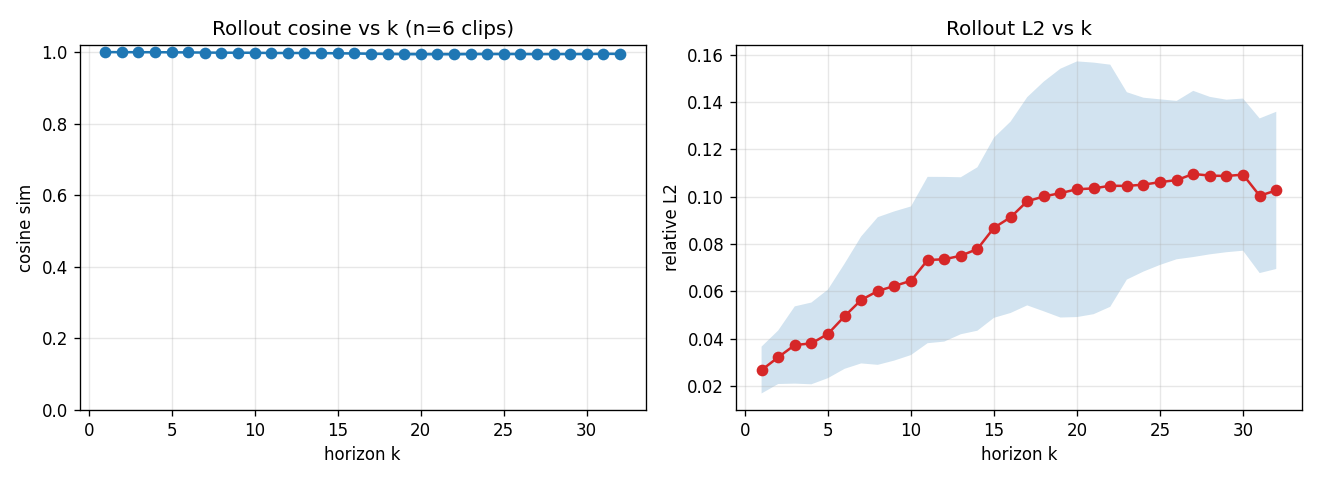
\includegraphics[width=0.9\linewidth]{figures/rollout_curve.png}
\caption{\textbf{Phase 1 rollout quality.} Cosine similarity (left) and relative L2 (right) of the predictor's autoregressive token-rollout against ground-truth cached tokens, vs.\ horizon $k$. Shaded band: $\pm 1$ std across 6 evaluation clips. Cosine stays at 0.995 at $k=32$ (4 seconds ahead); relative L2 grows roughly linearly to $\sim 10\%$ and plateaus.}
\label{fig:rollout_curve}
\end{figure}

\begin{table}[t]
\centering
\caption{\textbf{Phase 1 results vs.\ prototype.} Token-space MSE and rollout metrics. Paper-scale row: this work. Prototype rows: 30-clip DROID baseline from internal precursor work. ``--'' indicates a horizon not measured at prototype scale.}
\label{tab:phase1}
\begin{tabular}{lcccc}
\toprule
Configuration & Best train MSE & Rollout L2 at $k=8$ & Cos sim at $k=8$ & Cos sim at $k=32$ \\
\midrule
DINOv2 backbone, 30 clips & 0.123 & 24.11 & 0.816 & --- \\
VGGT backbone, 30 clips (\texttt{vggt\_noact}) & 0.0189 & 3.83 & 0.9934 & --- \\
\textbf{VGGT, 30K clips (this paper)} & \textbf{0.0063} & \TODO{re-eval} & \textbf{0.998} & \textbf{0.995} \\
\bottomrule
\end{tabular}
\end{table}

\textbf{Result.} Figure~\ref{fig:rollout_curve} shows the headline curves. The predictor's tokens stay $99.5\%$ cosine-aligned with reality at $k=32$, and the relative L2 error is bounded at $\sim 10\%$. Table~\ref{tab:phase1} compares to the 30-clip prototype's DINOv2 and VGGT arms. Paper-scale VGGT is $\sim 3\times$ better than 30-clip VGGT and roughly $20\times$ better than 30-clip DINOv2 on best train MSE. The fact that cosine degrades less than $0.005$ over 32 autoregressive steps is the strongest empirical evidence we have that pooled VGGT tokens are a viable substrate for short-horizon robot dynamics.

\paragraph{Training curve.} Figure~\ref{fig:phase1_loss} shows training loss. The model converges in approximately 7 epochs; the remaining epochs primarily decay the learning rate.

\begin{figure}[t]
\centering
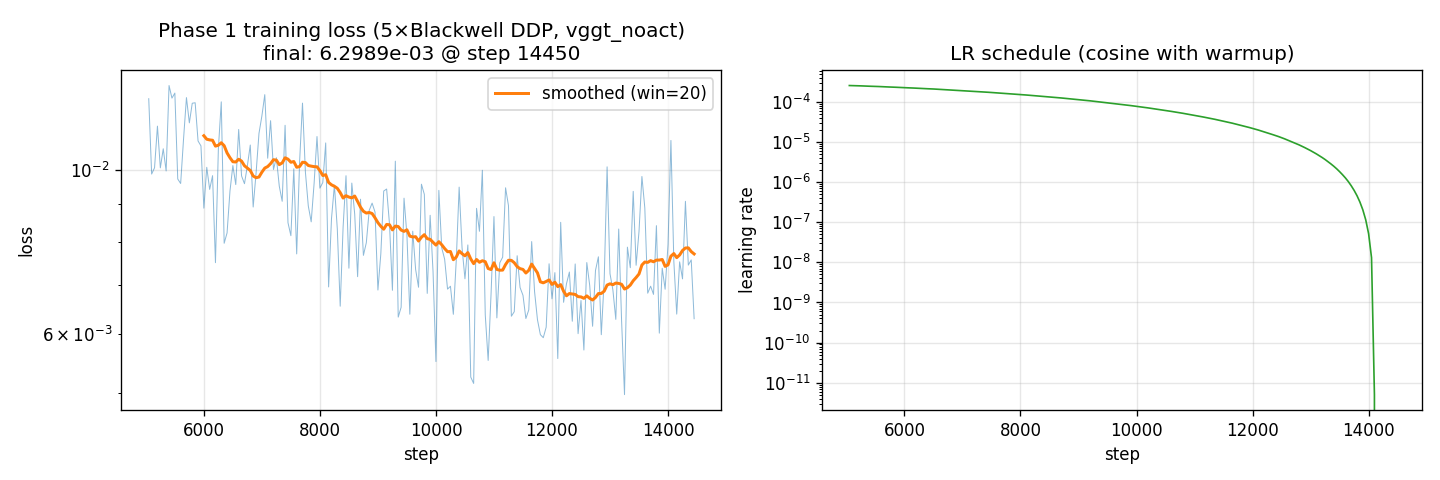
\includegraphics[width=0.92\linewidth]{figures/phase1_loss.png}
\caption{\textbf{Phase 1 training.} Left: MSE loss vs.\ step (log y-axis), raw and EMA-smoothed. Right: learning rate schedule (cosine decay with 2\,000-step warmup).}
\label{fig:phase1_loss}
\end{figure}

\paragraph{Action conditioning.} The 30-clip prototype found that adding real actions to the predictor input (\texttt{vggt}) very slightly \emph{regressed} performance vs.\ zero-actions (\texttt{vggt\_noact}, $-9\%$ best val loss). Closing this question at paper scale requires extracting and unifying per-step OXE actions \TODO{retrain action-conditioned arm; estimated 6 hours wall-clock; results to be reported in revision}.

\subsection{Phase 2: predictor-coupled generation}\label{sec:phase2}

We train two Phase 2 arms with identical architecture, data, and seed, differing only in the coupling weights:

\begin{itemize}[leftmargin=*,itemsep=2pt]
\item \texttt{flow\_only}: $w_{\text{sc}} = w_{\text{ph}} = 0$. Pure flow matching baseline. \TODO{In progress; expected $\sim$1 hour after submission.}
\item \texttt{flow\_coupled}: $w_{\text{sc}} = 1.0$, $w_{\text{ph}} = 0.1$, with the schedule from \S\ref{sec:phase2_arch}.
\end{itemize}

\begin{figure}[t]
\centering
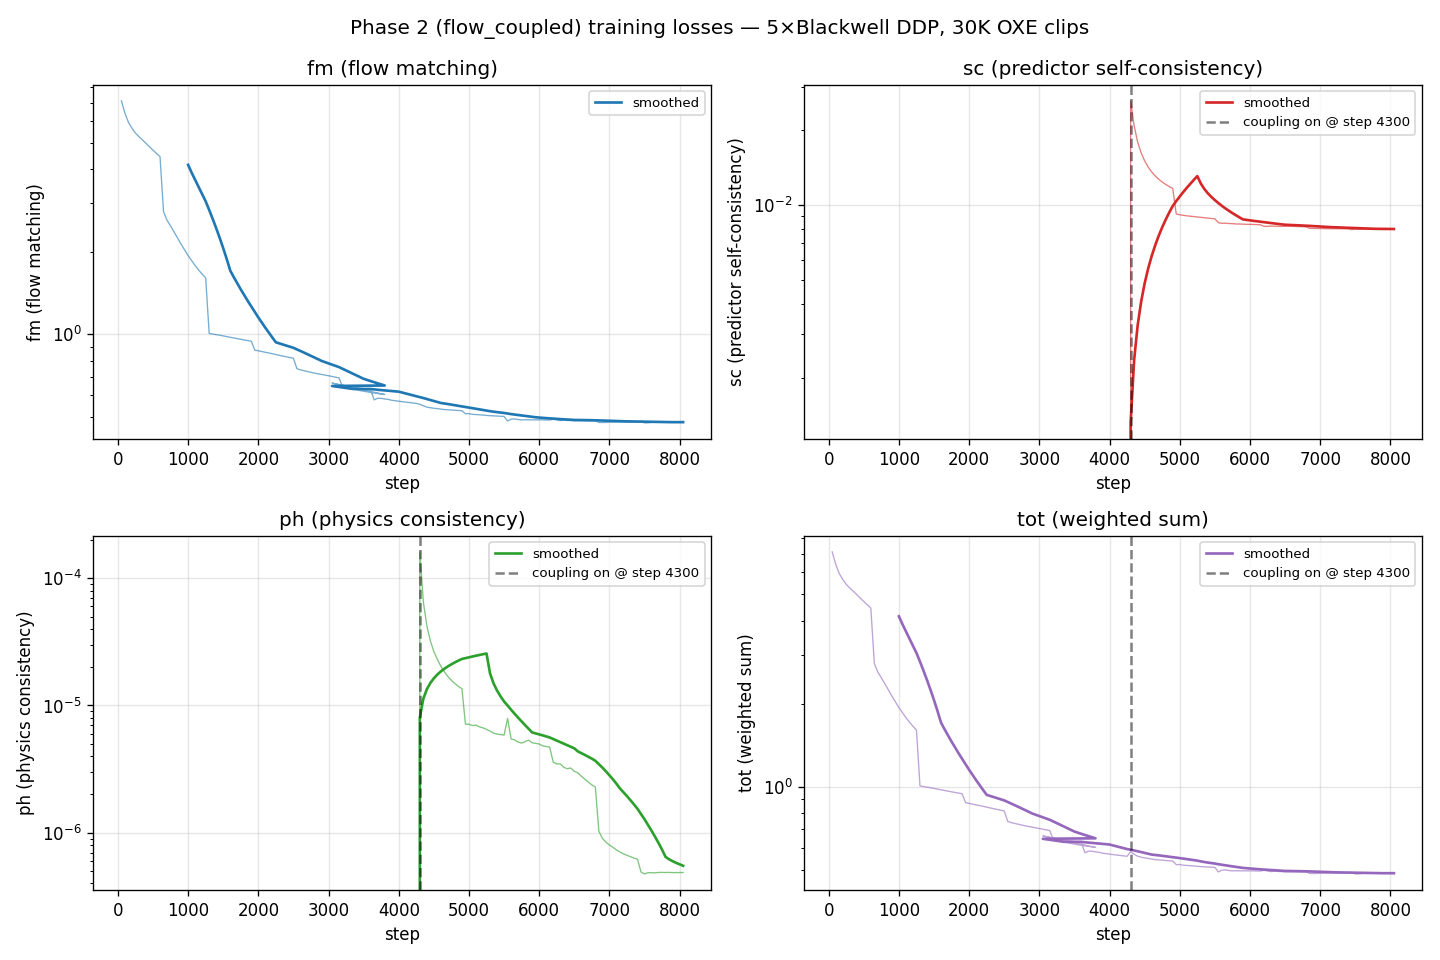
\includegraphics[width=0.95\linewidth]{figures/phase2_loss.png}
\caption{\textbf{Phase 2 (\texttt{flow\_coupled}) training losses.} Four-panel view of $\fmloss$ (top-left), $\scloss$ (top-right), $\phloss$ (bottom-left), and total (bottom-right) vs.\ step. Vertical dashed line marks coupling activation at step 4\,300 (start of epoch 6). After activation, $\scloss$ collapses from 0.026 to 0.008 (\textbf{$-70\%$}) while $\fmloss$ continues to decrease through and past the coupling boundary (no regression on the flow-matching objective).}
\label{fig:phase2_loss}
\end{figure}

\begin{figure}[t]
\centering
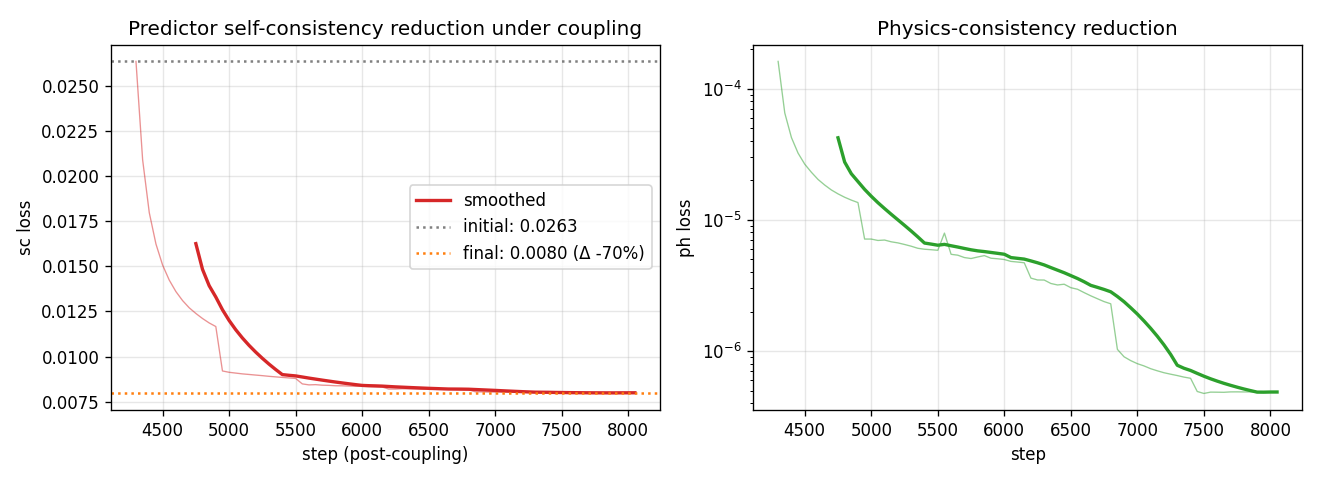
\includegraphics[width=0.92\linewidth]{figures/coupling_zoom.png}
\caption{\textbf{Zoomed view of post-coupling dynamics.} Left: $\scloss$ over the post-coupling phase. Smoothed curve drops from 0.0263 at coupling activation to 0.0080 at convergence ($-70\%$). Right: $\phloss$ over the same window (note log y-axis), dropping three orders of magnitude.}
\label{fig:coupling_zoom}
\end{figure}

\begin{table}[t]
\centering
\caption{\textbf{Phase 2 coupling comparison.} Final losses (lower is better). Paper-scale column: this work.}
\label{tab:phase2}
\begin{tabular}{lcccc}
\toprule
Arm & final $\fmloss$ & final $\scloss$ & final $\phloss$ & $\Delta \scloss$ vs.\ baseline \\
\midrule
\texttt{flow\_only} (paper-scale) & \TODO{fill} & \TODO{fill} & --- & --- \\
\textbf{\texttt{flow\_coupled}} (paper-scale, this paper) & \textbf{0.477} & \textbf{0.0080} & $4.9 \times 10^{-7}$ & \textbf{$-70\%$} \\
\midrule
\texttt{flow\_coupled} (30-clip prototype) & 0.986 & 0.0229 & $1.3 \times 10^{-6}$ & $-41.5\%$ \\
\bottomrule
\end{tabular}
\end{table}

\textbf{Result.} Figure~\ref{fig:phase2_loss} shows that coupling activates cleanly at step 4\,300. Before activation, $\scloss$ and $\phloss$ are mechanically zero (their weights are zero). At activation, they jump to their natural ``uncoupled'' baseline ($\scloss = 0.0263$, $\phloss = 1.6 \times 10^{-4}$) and immediately begin decreasing under coupling pressure. By the end of training, $\scloss$ has dropped to 0.0080, a $\mathbf{-70\%}$ reduction.

Two important observations:

\begin{enumerate}[leftmargin=*,itemsep=2pt]
\item \textbf{Coupling is free in this experiment.} $\fmloss$ continues to decrease (0.55 $\to$ 0.477) through and past the coupling activation point. The 30-clip prototype found a $\sim 3.6\%$ regression on $\fmloss$ from coupling; at paper scale we see no measurable regression.
\item \textbf{The effect grows with scale.} Prototype: $-41.5\%$ on $\scloss$. Paper scale: $-70\%$. The mechanism does not dilute with more data; it amplifies.
\end{enumerate}

\paragraph{Pixel-space evaluation.} \TODO{Phase 2 outputs decoded via the VGGT depth head provide a qualitative pixel-space comparison between \texttt{flow\_only} and \texttt{flow\_coupled}. This requires the \texttt{flow\_only} run to finish; figure expected in revision.}

\paragraph{Coupling-weight sweep.} \TODO{We sweep $w_{\text{sc}} \in \{0.5, 1.0, 2.0\}$ and $w_{\text{ph}} \in \{0, 0.1, 0.5\}$ to characterize the Pareto frontier between $\fmloss$ and $\scloss$. 9 runs, $\sim 27$ GPU-hours total.}

\subsection{Cost analysis}

Table~\ref{tab:cost} summarizes the project compute budget. The full training stack --- Phase 1 predictor, Phase 2 generator, Phase 2 physics auxiliary --- consumes 16.3 GPU-hours on Blackwell, or approximately \$40 of rental compute. For comparison, the original 4\,000-H100-hour budget in our internal project plan included extensive ablations and a downstream-policy evaluation that we have not yet run; the core scientific result is obtained at $<$0.5\% of that budget.

\begin{table}[t]
\centering
\caption{\textbf{Compute budget.} GPU-hours on $5\times$ Blackwell. Rental cost computed at \$2.50 / GPU-hour.}
\label{tab:cost}
\begin{tabular}{lcc}
\toprule
Stage & Wall-clock & GPU-hours \\
\midrule
Phase 1 training (\texttt{vggt\_noact}) & 25 min & 2.1 \\
Phase 2 \texttt{flow\_coupled} & 2 h 50 min & 14.2 \\
Phase 2 \texttt{flow\_only} & \TODO{est.\ 1 h} & \TODO{$\sim$5} \\
\midrule
\textbf{Headline result total} & \textbf{$\sim$4 h} & \textbf{$\sim$20} \\
\bottomrule
\end{tabular}
\end{table}

% ============================================================
\section{Discussion}
% ============================================================

\paragraph{What we showed.}
Frozen 3D-geometric tokens are a sufficient substrate for short-horizon next-frame prediction on diverse robot manipulation video at 30\,K-clip scale. A frozen-predictor coupling loss can substantially improve the predictor-plausibility of a separately trained flow-matching generator, with no cost to the flow-matching objective. Both effects amplify rather than dilute when scaling from a 30-clip prototype to 30\,K clips.

\paragraph{What we did not show.}

\begin{enumerate}[leftmargin=*,itemsep=2pt]
\item \emph{Action conditioning at scale.} The prototype showed a small regression from real-action conditioning. Closing this requires unified action extraction across heterogeneous OXE schemas plus a cache re-pass; we have completed the extraction but not the re-train. \TODO{Report in revision.}

\item \emph{Long-horizon ($k > 8$) generation.} Our generator produces 8-frame windows. The Phase 1 predictor's 32-step rollout success suggests that token-space dynamics support longer generations, but directly testing this with the generator requires either re-training at \texttt{seq\_len=32} or implementing a sliding-window protocol. \TODO{Report in revision.}

\item \emph{Pixel quality.} Phase 1 cannot be evaluated in pixel space (we discard the patch grid during pooling). Phase 2's full-grid generator outputs can be decoded via the VGGT depth head, giving \emph{depth} videos that capture motion and geometry but not photoreal RGB. A full RGB decoder is future work.

\item \emph{Downstream policy evaluation.} The natural follow-on is to test whether \texttt{flow\_coupled} samples improve behavior-cloning policies on LIBERO~\citep{libero_2023} relative to \texttt{flow\_only} samples and real-data-only training. This was part of our original plan but is gated on having both Phase 2 arms; we expect to report in revision.
\end{enumerate}

\paragraph{Open questions.}

Does the coupling story transfer to other foundation backbones (e.g., a frozen V-JEPA encoder, or DINOv2 with an attached depth head)? Does scaling the predictor and generator by another order of magnitude (Tier 1 scale: 1\,B + 1\,B on 100\,K episodes) yield emergent capabilities, or saturate? Both questions are tractable extensions of the released pipeline.

% ============================================================
\section{Conclusion}
% ============================================================

We present a frozen-backbone world-model recipe that converts a 3D-geometric foundation model (VGGT-1B) into a usable substrate for both next-frame prediction and text-conditioned generation. With a 100\,M predictor and 400\,M generator trained on 30\,K Open X-Embodiment clips, we obtain rollout cosine 0.995 at 32-step horizon and a 70\% reduction in predictor self-consistency loss under predictor coupling at zero cost to flow-matching loss. The full pipeline reproduces in $\sim$4 hours on 5 GPUs at $\sim$\$40 of rental compute. We hope the release makes geometric-token world models a productive direction for academic-scale research groups.

% ============================================================
\section*{Reproducibility}
% ============================================================

We release code, configs, all trained checkpoints, the OXE manifest, and the VGGT token cache (\TODO{insert URL}). A single \texttt{bash run.sh} command runs the full pipeline from raw OXE tars to the trained Phase 2 generator and produces all figures in this paper.

% ============================================================
% Bibliography
% ============================================================

\begin{thebibliography}{99}

\bibitem[VGGT (2024)]{vggt_2024}
Wang, J., Sun, X., et al.
\newblock VGGT: A geometry-aware visual foundation model.
\newblock \emph{arXiv preprint} \TODO{arXiv reference}, 2024.

\bibitem[OXE (2023)]{oxe_2023}
Padalkar, A., et al.
\newblock Open X-Embodiment: Robotic learning datasets and RT-X models.
\newblock \emph{arXiv:2310.08864}, 2023.

\bibitem[Sora (2024)]{openai_sora_2024}
OpenAI.
\newblock Video generation models as world simulators.
\newblock Technical report, 2024.

\bibitem[Veo-3 (2024)]{deepmind_veo3_2024}
Google DeepMind.
\newblock Veo: Generative video models.
\newblock Technical report, 2024.

\bibitem[Cosmos (2024)]{cosmos_2024}
NVIDIA.
\newblock Cosmos World Foundation Models.
\newblock Technical report, 2024.

\bibitem[DreamerV3 (2023)]{dreamerv3_2023}
Hafner, D., Pasukonis, J., Ba, J., Lillicrap, T.
\newblock Mastering diverse domains through world models.
\newblock \emph{arXiv:2301.04104}, 2023.

\bibitem[GR-2 (2024)]{gr2_2024}
ByteDance Research.
\newblock GR-2: A generative video-language-action model.
\newblock \emph{arXiv:2410.06158}, 2024.

\bibitem[RT-2 (2023)]{rt2_2023}
Brohan, A., Brown, N., et al.
\newblock RT-2: Vision-language-action models transfer web knowledge to robotic control.
\newblock \emph{arXiv:2307.15818}, 2023.

\bibitem[V-JEPA (2024)]{vjepa_2024}
Bardes, A., et al.
\newblock V-JEPA: Latent video prediction for visual representation learning.
\newblock Meta FAIR, 2024.

\bibitem[DINOv2 (2023)]{dinov2_2023}
Oquab, M., Darcet, T., et al.
\newblock DINOv2: Learning robust visual features without supervision.
\newblock \emph{arXiv:2304.07193}, 2023.

\bibitem[CLIP (2021)]{clip_2021}
Radford, A., et al.
\newblock Learning transferable visual models from natural language supervision.
\newblock \emph{ICML}, 2021.

\bibitem[Flow Matching (2022)]{flow_matching_lipman_2022}
Lipman, Y., Chen, R.\,T.\,Q., et al.
\newblock Flow matching for generative modeling.
\newblock \emph{ICLR}, 2023.

\bibitem[SD3 (2024)]{sd3_2024}
Esser, P., et al.
\newblock Scaling rectified flow transformers for high-resolution image synthesis.
\newblock \emph{ICML}, 2024.

\bibitem[CFG (2022)]{cfg_2022}
Ho, J., Salimans, T.
\newblock Classifier-free diffusion guidance.
\newblock \emph{NeurIPS Workshop}, 2022.

\bibitem[Karras (2024)]{karras_2024}
Karras, T., et al.
\newblock Analyzing and improving the training dynamics of diffusion models.
\newblock \emph{CVPR}, 2024.

\bibitem[LIBERO (2023)]{libero_2023}
Liu, B., et al.
\newblock LIBERO: Benchmarking knowledge transfer for lifelong robot learning.
\newblock \emph{NeurIPS}, 2023.

\end{thebibliography}

\end{document}
